\section{Transport and strict ordering of the optimal value}\label{sec:transport}
The coefficient derivatives in \eqref{eq:coefficientmotion} and a uniform
remainder suffice to compare well-separated parameters. They do not by
themselves compare the actual values at arbitrarily close parameters.
We use a change of scale which preserves all the moment equations.
Weighted composition operators on Lipschitz spaces are an established
framework \cite{abbar}; the result below is a sufficient differential
condition adapted to these moments and to a specified amplitude-to-slope
ratio.

\begin{theorem}[Moment-preserving transport]\label{thm:transport}
Suppose \(w_\nu(u)>0\) is \(C^2\) in \(u\), is \(C^1\) in \(\nu\),
and has continuous mixed derivative \(\partial_u\partial_\nu\log w_\nu\).
Suppose \(f_\nu>0\) and \(\tau(\nu)>0\) are \(C^1\).
Assume that the following kernels are integrable on the half-line:
\[
 q_{j,\nu}(u)=w_\nu(u)(2u)^j
                 \cos(2\tau(\nu)u+j\pi/2),\quad 0\leq j\leq m .
\]
Let \(\kappa=-\tau'/\tau\geq0\), \(L_\nu=\partial_u\log w_\nu\), and
\[
 r_\nu(u)=-f_\nu'/f_\nu+(m+1)\kappa
               +\partial_\nu\log w_\nu(u)+\kappa uL_\nu(u).
\]
If for constants \(a_0,c>0\)
\begin{equation}\label{eq:transportcriterion}
 r_\nu+\kappa+a_0|\partial_ur_\nu|\leq-c
\end{equation}
throughout a parameter interval and the whole half-line, then for
\(\nu_1<\nu_2\), \(d=\nu_2-\nu_1\), \(\eta=\tau(\nu_1)/\tau(\nu_2)\),
the transformation
\begin{equation}\label{eq:transportmap}
 (\mathcal T g)(u)=T(u)g(\eta u),\qquad
 T(u)=\frac{f_{\nu_1}}{f_{\nu_2}}\eta^{m+1}
                 \frac{w_{\nu_2}(\eta u)}{w_{\nu_1}(u)}
\end{equation}
preserves feasibility of the moment equations from \(\nu_2\) to \(\nu_1\).
If \(\norm{g}_\infty\leq a_0M\), \(\Lip(g)\leq M\), then
\[
 \norm{\mathcal T g}_\infty\leq e^{-cd}\eta^{-1}\norm{g}_\infty,
 \qquad \Lip(\mathcal T g)\leq e^{-cd}M .
\]
Consequently, whenever the optimum at \(\nu_2\) is attained with
amplitude at most \(a_0M\),
\begin{equation}\label{eq:order}
 \delta_{\nu_2}(M)\geq\eta e^{cd}\delta_{\nu_1}(M).
\end{equation}
\end{theorem}
\begin{proof}
Substitution \(x=\eta u\) and
\(p_{j,\nu_2}(\eta u)=\eta^jp_{j,\nu_1}(u)\) give the exact identity
\[
 \int q_{j,\nu_1}\mathcal T g
   =\frac{f_{\nu_1}}{f_{\nu_2}}\eta^{m-j}\int q_{j,\nu_2}g .
\]
This proves all moments, including the target at \(j=m\).

For the norm estimate, set \(\nu(t)=\nu_2-t\) and
\(\eta(t)=\tau(\nu(t))/\tau(\nu_2)\), and use \eqref{eq:transportmap}
with this moving first endpoint. Define
\(\mathcal D=\partial_t-\kappa u\partial_u\).
Direct logarithmic differentiation gives
\[
 \mathcal DT=rT,\qquad \eta'=\kappa\eta,\qquad
 \mathcal D(T_u)=(r+\kappa)T_u+r_uT .
\]
The positive commutator term \(+\kappa T_u\) is essential.
Since \(\eta\geq1\), \(T>0\), the quantity
\(W=\eta T+a_0|T_u|\) satisfies \(T\leq W\), and, along each
characteristic,
\[
 \mathcal DW\leq(r+\kappa)W+a_0|r_u|T\leq-cW .
\]
The inequality for the absolute value is valid almost everywhere;
alternatively it follows by regularization. Initially \(T=1,T_u=0\),
so \(W(0,u)=1\). Every finite endpoint characteristic has a finite
initial point. Thus no uniform boundedness of \(r\) at infinity is
needed, and
\[
 \eta T+a_0|T_u|\leq e^{-ct},\qquad T\leq e^{-ct}/\eta .
\]
The product and chain rules for Lipschitz functions prove the two norm
bounds. Applying them to an optimizer at \(\nu_2\) provides a feasible
competitor at \(\nu_1\) and proves \eqref{eq:order}.
\end{proof}

\begin{corollary}[Strict order on the theta branch]\label{cor:thetaorder}
For the family in Section~\ref{sec:theta}, for every \(M\geq2\cdot10^{-5}\)
and every \(-1/64\leq\nu_1<\nu_2\leq0\),
\begin{align}
 \delta_{\nu_2}(M)
 &\geq\frac{\tau(\nu_1)}{\tau(\nu_2)}
          e^{(\nu_2-\nu_1)/50}\delta_{\nu_1}(M)
  >\delta_{\nu_1}(M),\label{eq:thetaorder}\\
 \log\delta_{\nu_2}(M)-\log\delta_{\nu_1}(M)
 &>0.02259(\nu_2-\nu_1),\nonumber\\
 \delta_{\nu_2}(M)-\delta_{\nu_1}(M)
 &>2.07\cdot10^{-11}(\nu_2-\nu_1).\label{eq:linearorder}
\end{align}
These inequalities do not require differentiability or uniqueness of
the finite-budget optimizer.
\end{corollary}
\begin{proof}
The validated branch bounds include
\[
 .00259<\kappa<.00260,\quad .0437<f_\nu'/f_\nu<.0451,
 \quad .3260<\lambda'<.3264,\quad .2939<\mu'<.2942 .
\]
With \(a_0=2^{-14}\), Appendix~\ref{app:transport} proves
\eqref{eq:transportcriterion} with \(c=1/50\) on the whole half-line.
Theorem~\ref{thm:theta} gives
\(\delta_\nu(M)/M<9.181\cdot10^{-10}/(2\cdot10^{-5})<a_0\),
so Theorem~\ref{thm:transport} applies. Integrating the strict lower
bound for \(\kappa\) proves the logarithmic bound.
Finally \(e^x-1\geq x\) and
\(9.17\cdot10^{-10}\cdot.02259>2.07\cdot10^{-11}\)
give \eqref{eq:linearorder}.
\end{proof}

For a fixed nonzero separation, the coefficient bounds can give a sharper
two-sided estimate. Integrating \eqref{eq:coefficientmotion} and subtracting
the two errors in \eqref{eq:thetaerror} gives, with \(d=\nu_2-\nu_1\),
\[
 \mathcal L(M)d-\frac{2.66\cdot10^{-53}}{M^6}
 <\delta_{\nu_2}(M)-\delta_{\nu_1}(M)
 <\mathcal U(M)d+\frac{2.66\cdot10^{-53}}{M^6},
\]
where
\begin{align*}
 \mathcal L(M)&=2.7\cdot10^{-11}+7.4\cdot10^{-26}M^{-2}
                              +1.9\cdot10^{-40}M^{-4},\\
 \mathcal U(M)&=3.0\cdot10^{-11}+8.7\cdot10^{-26}M^{-2}
                              +5.3\cdot10^{-40}M^{-4}.
\end{align*}
The transport estimate remains strictly positive however small \(d>0\)
is; the fixed error allowance in the two-sided estimate cannot do this.

\begin{figure}[tb]
 \centering
 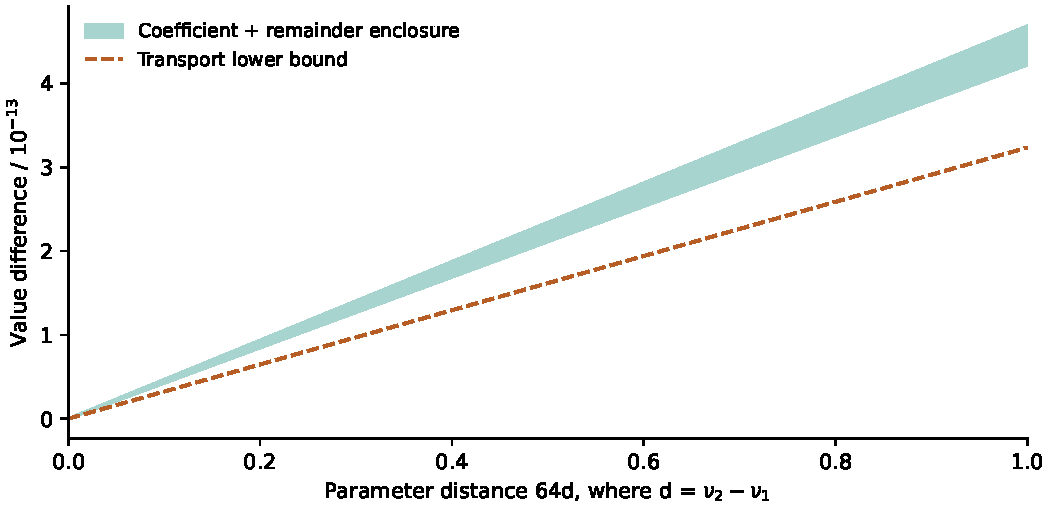
\includegraphics[width=.86\linewidth]{figures/theta_comparison.pdf}
 \caption{Guaranteed bounds on the change of the optimal value at
 \(M=2\cdot10^{-5}\), for any two driver parameters at distance \(d\).
 The shaded region is the coefficient-plus-remainder enclosure derived
 in this section.
 The dashed line is the weaker but strictly positive transport bound
 \(2.07\cdot10^{-11}d\). This plot displays bounds, not numerically
 computed finite-budget optimizers. At \(d=0\) the exact difference is zero.}
\end{figure}
